\documentclass{article}
\usepackage[UKenglish]{babel}
\usepackage{url}
\usepackage[T1]{fontenc}
\usepackage{lineno} % used in genre
\usepackage{booktabs}
\usepackage{graphicx}
\usepackage{setspace}
\usepackage{tabularx}
\usepackage{multicol}
\usepackage{comment}
\usepackage{graphics}
\usepackage[hidelinks]{hyperref}

\usepackage[backend=biber,style=apa,apamaxprtauth=7,doi=false,isbn=false,uniquename=false,url=false,bibencoding=utf8]{biblatex}
\DeclareLanguageMapping{british}{british-apa}

% no notes ??
\AtEveryBibitem{%
  \clearfield{note}%
}
\usepackage{xparse}
\usepackage{csquotes}
\usepackage[open]{bookmark}

\addbibresource{references.bib}

% i will stop using this soon.
% it allows old style citing
\newcommand{\citeNP}{\cite}
\renewcommand{\cite}{\parencite}

% make sure there's a comma after and in refs like proper apa
\AtBeginDocument{\renewcommand\finalandcomma{\addcomma}}
\AtBeginBibliography{%
  \renewcommand*{\finalnamedelim}{%
    \ifthenelse{\value{listcount}>\maxprtauth}
      {}
      {\finalandcomma\addspace\&\space}}}


\author{Daniel McDonald}
\date{\today}
\title{Diagnosis discourses in an online bipolar community: a corpus linguistic exploration}

\begin{document}

\maketitle

\section{Context}

Innumerable online support groups (OSGs) exist today online. In these spaces, both those living with health problems and those who care for them exchange both social support and health information.

These communities are generally text- and forum-based

A decreasing popularity of forums has led to OSGs appearing within other kinds of site architectures, such as subreddits.

Communities vary a great deal in terms of their demographics (with many )

Moreover, forum rules and cultures vary significantly: communities may require users to stay anonymous, to have or not have official diagnoses, 

The ratio of sufferers to friends and family thereof can also vary,.

Anonymous text-based forums can be quickly and automaticaly turned into corpora for linguistic analysis. Many forums are also metadata-rich, with easily extractable information such as timestamps, genders, usernames, numbers of posts, and so on.

\section{Literature review}



Despite the dozens of studies of online communities, a major currently shortcoming is a difficulty in translating these findings into policy and practice suggestions.

\subsection{Online health communities}

\subsection{Diagnosis}

\subsection{Language-centred approaches to health discourse}

Qualitative, quantitative and mixed-methods paradigms have all been used in the study of OSGS.

Qualitative-only investigations provide rich accounts of lived experience, and often do a better job of understanding the motivations of a single community member. These approaches, however, are difficult

Because they cannot be automated, they cannot be automatically re-performed on new datasets.This further limits reproducibility.

Finally, qualitative approaches may be of limited use in informing policy and practice in mainstream medicine.

Corpus-based methods provide a means of ameliorating some of these concerns. With corpora, it is possible to analyse all contributions to one or many health communities, making possible generalisations about how community members, or subsets thereof, typically use language.

At the same time, it is important to bear in mind that corpus frequencies alone can obscure the kinds of insights that come from sustained, contextualised analysis.

Corpus approaches often consider clauses or words in isolation from the full text in which they were produced.

Finally, typical corpus methods are often well behind the computational state-of-the-art.

%\subsection{Emerging methods for analysing large, digital collections of text}

Corpus linguistics, as an approach, often consists of a more-or-less standard set of practices, such as concordancing, keywording, and collocate analysis. Computational linguistics, meanwhile, has developed far more sophisticated methods for automating analysis of text. Well-written English can be annotated and parsed using a number of grammatical frameworks.

More recently still, the turn toward statistical NLP has seen a reduced focus on human-developed grammars.

If a researcher is interested in topics typically discussed by new members, for example, he\slash she can manually annotate a set of posts, and employ a machine learning algorithm to group remaining posts into this scheme. By withholding a selection of manually annotated posts during training, the researcher can then run the model on the withheld data in order to score its overall accuracy.

\section{Case study}



\section{Findings and discussion}


\subsection{Qualitative exploration}

\begin{quote}
\resetlinenumber
\footnotesize{
\singlespacing{
\begin{linenumbers}
\begin{verbatim}
hi im jess new to this site, umm... well im currently 20 years 
old and have been diagnosed with depression from a young age 
but in the last 5 years or so i have been feeling very odd having 
some extreme highs which include loss of appetite concentration
using drugs and alcohol spending sprees and also sex, i can not 
control this when i get impulses like the above it is impossible 
though i have tried. I also suffer with depression which is quite
severe most of the time i find it hard to get out of bed or to 
even be able to connect with anyone including my partner who 
lives with me, i am hurting him so much but i dont feel like i 
can do anytjing about it
    i have asked my doctor to test me to see if i am bipolar as my 
antidepressants do not work even though they have been changed a 
million times!! he said no that he wont test me and i also asked 
for counselling and he also declined that, at the moment i feel 
that im loosing control of everything and its getting worse, i 
want to change my doctor and have been telling my partner i would 
but im scared of finding out that i am bipolar, but i really feel 
like either an extreme high or an extreme low is on the way and 
im quite scared i dont know what to do
    please help \end{verbatim}
\end{linenumbers}
}}
\end{quote}

The post is reminiscent in form and function to post analysed in other work on OSG: Jess indicates a need for general social support (\emph{im quite scared}, line 20) and requests advice (\emph{what should i do?}, title; \emph{i dont know what to do}, line 21). As noted by \textcite{smithson_developing_2012} and \textcite{varga2014grieving}, in order to legitimate herself as a potential member, and add perlocutionary force to her request, Jess also offers a narrative designed to demonstrate that she likely suffers from bipolar, and thus fulfills the membership criteria of the board. Also notable is the sense of urgency, which has been conveyed through an apparent lack of planning within the post, spelling errors (\emph{anytjing}, line 11; \emph{loosing control}, line 17), and the pervasive joining of clauses through conjunction. As noted by \textcite{horne_doing_2009}, this may be a strategy for increasing the likelihood of response. In the context of bipolar disorder, it could also connote the onset of a manic episode, which would serve to bolster the claim to membership.

\subsubsection{Generic stages in Jess first post}

The post appears to borrow from both \textsc{self-introduction} and \textsc{narrative} genres identified by \textcite{labov_narrative_1997}. Indeed, in many ways, the post conforms to the \textsc{narrative} genre, which has the structure:

\begin{quote}
(Abstract) $\hat{}$ Orientation $\hat{}$ Complication $\hat{}$ Evaluation $\hat{}$ Resolution $\hat{}$ (Coda)
\end{quote}

\noindent where

\begin{itemize}\onehalfspacing{
\item \textsc{Abstract} is an encapsulation of the point of the story
\item \textsc{Orientation} orients the listener to the circumstances of the story
\item \textsc{Complication} is temporally sequenced event which culminates in a problem
\item \textsc{Evaluation} is the attitude of the speaker toward the \textsc{complication}
\item \textsc{Resolution} is how the story's protagonist resolved the \textsc{complication}
\item \textsc{Coda} makes a point about the text and may reorient the listener to the present \cite[p.~32]{labov_narrative_1997}.
}
\end{itemize}
%
As shown in Table \ref{jess-genre}, the \textsc{abstract} stage is realised by the post's title; \textsc{orientation}, \textsc{complication} and \textsc{evaluation} do follow, though they appear to be recursive. Also different is the focus of the \textsc{evaluation}: here, it refers to an \textsc{evaluation} of the previous complication, rather than an evaluation of the narrative itself. The most significant deviation is that rather than a \textsc{resolution} (and optional \textsc{coda}), there is a \textsc{request} to other members for `help', presumably with the questions posted in the title: whether or not she is bipolar, and how she should respond to her presented self-evaluation.

\begin{table}[htb]\centering\small
\begin{tabularx}{\textwidth}{lX}

\toprule
Genre stage  & Sentences in Jess's first post   \\ \midrule
\textsc{Abstract }    & am i bipolar and what should i do? \\ 
\textsc{Salutation}   & hi im jess   \\ 
\textsc{Orientation}  & (I am) new to this site,  umm... well im currently 20 years old and (I) have been diagnosed with depression from a young age but \\ 
\textsc{Complication (1)} & in the last 5 years or so i have been feeling very odd, (I have been) having some extreme highs which include loss of appetite concentration using drugs and alcohol spending sprees and also sex, \\ 
\textsc{Evaluation (1)}   & i can not control this when i get impulses like the above it is impossible though i have tried \\ 
\textsc{Complication (2)} & I also suffer with depression which is quite severe most of the time i find it hard to get out of bed or to even be able to connect with anyone including my partner who lives with me,   \\ 
\textsc{Evaluation (2)}   &  i am hurting him so much but i dont feel like i can do anytjing about it   \\ 
\textsc{Complication (3)} & i have asked my doctor to test me to see if i am bipolar as my antidepressants do not work even though they have been changed a million times!! he said no that he wont test me and i also asked for counselling and he also declined that, \\ 
\textsc{Evaluation (3)} & at the moment i feel that im loosing control of everything and its getting worse, \\ 
\textsc{Complication (4)} &  i want to change my doctor and (I) have been telling my partner i would but im scared of finding out that i am bipolar, but  \\ 
\textsc{Evaluation (4)}   & i really feel like either an extreme high or an extreme low is on the way and im quite scared i dont know what to do  \\ 
\textsc{Request}     & please help   \\ \bottomrule
\end{tabularx}
\caption{Genre stages in Jess's post}
\label{jess-genre}
\end{table}
%
Within a possible `first-post genre', explicit \textsc{Requests} are potentially optional \cite{vayreda_social_2009}, though other members may interpret descriptions of problems and the act of posting themselves as warranting the provision of advice \cite{goldsmith2000soliciting}. Some researchers \cite[e.g. ][]{herring_two_1996,weber_missed_2011} have noted that member{users} may not begin introductions to online communities with an explicit \textsc{salutation}: as all messages are attributed to the writer's username multimodally, and even new member{users} are likely familiar with the way in which the site presents post, \textsc{salutation}, if not rendered explicitly in prose, is in some sense embedded within the architecture of the forum mode itself. Given that all post must be titled, and that titles almost always summarise the content of the post, \textsc{Abstract} is an obligatory stage. The generic structure provided by \textcite{labov_narrative_1997} could thus be adapted for this case as:

\begin{quotation}\small
\noindent Abstract $\hat{}$ Salutation $\hat{}$ Orientation $\hat{}$ [ Complication $\hat{}$ Evaluation ]\textsuperscript{n} $\hat{}$ (Request)
\end{quotation}
%
To characterise the extent to which Jess's post was representative of the genre, the two first post with the smallest wordcount were located and a basic genre stage analysis was performed (Table \ref{tab:two-genre-stage-analyses}). It was assumed that small first post would contain only obligatory genre features. These short post indicate that \textsc{evaluation} is an optional stage, and confirm that recursion of \textsc{complication} and \textsc{evaluation} is optional (though perhaps a key feature in developing a sense of urgency). \emph{Short Post B} shows that the optional \textsc{coda} noted by \textcite{labov_narrative_1997} appears to be possible within the first-post genre. This leaves a finalised generic structure for thread-initial first post within the Bipolar Forum:

\begin{quotation}\small
\noindent Abstract $\hat{}$ Salutation $\hat{}$ Orientation $\hat{}$ [ Complication $\hat{}$ (Evaluation) ]\textsuperscript{n} $\hat{}$ (Request) $\hat{}$ (Coda)
\end{quotation}

\begin{table}[htb]
\small\centering
\begin{tabularx}{\textwidth}{lXX}
\toprule
Genre stage  & Sentences in Short Post A  & Sentences in Short Post B \\ \midrule
\textsc{Abstract}     & \emph{Lamictal}  & \emph{Depakote and hair thinning - any suggestions?}  \\
\textsc{Salutation}   & Hi-                                                                              & Hi                                                                      \\
\textsc{Orientation}  & I'm on my 3rd day of Lamictal and                                                & My daughter has been on Depakote for 4 months and                       \\
\textsc{Complication} & it's giving me weird almost headache like pains in my head                       & (she) has experienced some (h)air thinning                              \\
\textsc{Evaluation}   & ~                                                                                & ~                                                                       \\
\textsc{Request }     & Has anyone else had this happen while taking lamictal and when does it go away? & Has anyone out there found an effective way to counteract this problem? \\
\textsc{Coda}         & ~                                                                                & She is on 500mg per day. Any suggestions really appreciated.            \\
\bottomrule
\end{tabularx}
\caption{Genre stages in short first contributions}
\label{tab:two-genre-stage-analyses}
\end{table}
%
It is not enough, however, to simply look at the features of the post: as \textcite{eggins_analysing_2004} explain, perhaps the best indicator of genre conformity is the way in which other members respond to the presented text. Thus, at this point, the investigation turns to consider replies to Jess's first post.

\subsection{Replies to a first post}

Jess's first contribution received six replies over the course of seven hours, from member with post counts ranging from five to over 5,000. Due to limitations of scope, only two of these replies have been selected for further analysis. They were selected based on the post count of the writer at the time of posting: one is a newer user (Subcorpus 03) and the other is a very senior member (Subcorpus 10). They also bookend the replies: the newer user is the first to respond to Jess, and the veteran member the last. The qualitative analysis, therefore, provides a description of language use at multiple stages of the membership course. %The complete thread, including the other four replies, is available in Appendix \ref{appendix:thread}.

The first reply was a response from \emph{Luvsoccer}, who had a total of five post to the board:

\begin{quote}
\resetlinenumber
\footnotesize{
\singlespacing{
\begin{linenumbers}
\begin{verbatim}
It sounds like you might have bipolar to me. You need to change 
Drs. One with more knowledge apparently. The reason the 
antidepessants are not Working is because If you are bi polar 
and they put U on an antidepressant alone it can make things 
worse... I know from experience. Don't be scared it's treatable. 
Find you a dr that can make a correct Diagnosis and go from there. 
Good luck! \end{verbatim}
\end{linenumbers}
}}
\end{quote}
%
\noindent Following \emph{Luvsoccer} were four replies from other member at differing membership stages, unanalysed here. The final post in the thread was by \emph{Emz45}, who at the time of data collection had authored 5071 post:

\begin{quote}
\resetlinenumber
\footnotesize{
\singlespacing{
\begin{linenumbers}
\begin{verbatim}
Hi, welcome to the boards, hopefully we can help you out and be 
a support system for you. First off you're not A bipolar, *l* 
we're not things, it's a condition. From what you say, if 
sounds very likely that you might have Bipolar disoder. I would 
go to a psychiatrist for testing and find out. You don't have to 
have your docs permission to do this. If you're already seeing a 
psychiatrist and that's who's doing all the denying, then find a 
different one, because he's not doing his job, nor is he 
considering your best interest. That's all that you can really 
do in the beginning, find out what's what. We aren't docs here 
and can't diagnose you. But I think it would definitely be smart 
to go and get a diagnoses.

Take care, and please keep in touch, let us know how you're 
doing, okay?

Emz \end{verbatim}
\end{linenumbers}
}}
\end{quote}
%
\noindent The original poster did not contribute to the thread again, but posted to the board on three other occasions in the next week, interacting again with \emph{Emz45}.

\subsubsection{Analysis of replies} \label{sect:qual-reply-analysis}

A first notable feature of the replies is their functional similarity. Both Luvsoccer and Emz45 offer social support (\emph{Don't be scared}, line 5; \emph{take care}, line 14), and encourage Jess to find a new doctor. Both also hint at a likely diagnosis based on the symptoms she has presented. In both cases, key ideological tenets of the Forum are represented delicately. Both disparage the work of Jess's current psychiatrist (\emph{One with more knowledge}, line 2; \emph{he's not doing his job}, line 8). Both navigate the Forum's conflict between an inability to provide official diagnoses and an orientation toward supporting those who appear to have bipolar. In fact, both provide near-identical wordings:

\begin{enumerate}
\item \emph{It sounds like you might have bipolar to me}
\item \emph{From what you say, if sounds very likely that you might have Bipolar disoder}
\end{enumerate}
%
Both statements essentially amount to a lay diagnoses, with modulation, modalisation, embedding and dummy Subjects used to reduce certainty and to avoid attribution of the diagnosis to the speaker herself. Both further hedge the lay diagnosis by stressing the need for a professional diagnosis, and, in doing so, deny that what they offered was any kind of diagnosis at all.

%todo: first sentence doesn't make sense
The relationship between first-post and reply differ across the hierarchy of stratification. At the stratum of genre, unlike first post, the two replies do not conform rigourously to an identifiable sequence of clause functions. At the same time, the fact that the two responses overlap in content may be a useful indication that first post do constitute a genre that is recognised by other member of the community. In terms of register, while the dimension of Field remains largely consistent (aside from Emz's avoidance of the topic of specific medications), the most dramatic differences are within Tenor: Jess is a prototypical newcomer, describing a medical history and current problem, positioning herself as vulnerable, lacking agency, and unable to participate effectively in her own care. In contrast, to Jess's descriptions of the past and present, Luvsoccer and Emz offer explanations and potential actions for the future. 

Within the lexicogrammar, we can see differences in how the first and non-first-post construe reality via the system of \textsc{Transitivity}. All participants position themselves as Sensers, but the kinds of mental processes vary in their representation of subjectivity, reasoning and control. Jess characterised herself through subjective mental processes over which she has no agency (\emph{i have been feeling very odd}, \emph{i dont feel like i  can do anytjing about it}, \emph{i feel that im loosing control of everything}, \emph{i really feel like either an extreme high or an extreme low is on the way}); Luvsoccer, in contrast, \emph{know[s] from experience}, while Emz \emph{thinks} that diagnosis is the most important next step. Jess construes the health professional as an Agent, and most often, a Sayer (\emph{He said no}; \emph{He also declined that}), whose actions negatively affect her ability to obtain needed treatment. This contrasts with the other members, who reformulate health professionals as Goals (\emph{You need to change Drs}; \emph{Find you a dr}; \emph{I would go to a psychiatrist for testing}, etc.) Jess positions her partner, on the other hand, only as a Goal or Target, and never a Participant that puts processes in motion (\emph{i find it hard to [...] to connect with anyone including my partner}; \emph{i am hurting him so much}; \emph{I ... have been telling my partner}). For this reason, the partner is not construed at all in either response.

%Emz's advice provision strategy is to use modalisd material processes to show Jess the result of her reasoning: in \emph{I would go to a psychiatrist for testing and find out}, Emz foregrounds actions based on her familiarity with the situation.

There are also differences in the way first and non-first post instantiate the system of \textsc{Mood}. All of Jess's major Mood choices are declarative and congruently work to provide information, until a final imperative, \emph{please help}, which shifts the function of the post from the recursive narrative stages of \textsc{Orientation}, \textsc{Complication} and \textsc{Evaluation}, making a modulated demand on readers to address her declared fear and need for information (\emph{im quite scared i dont know what to do}). The Subject of most of Jess's clauses is \emph{I}, emphasising the self as the one invested with modal responsibility, and thus, the one who will honour any advice that others choose to provide. Modalisation of the self as Subject is used to stress an inability to modify behaviour (\emph{I can not control this}, \emph{I don't feel like I can do anything about it}). This is in contrast to the responses, which use interrogative and imperative Moods to request further information and to command the new user to respond. \emph{You} is by far the the most common Subject in the two replies, as the responses keep modal responsibility on Jess herself. Modalised declarative choices, meanwhile, do not always provide information, but may also issue directives in the form of advice: Emz does this twice, casting herself as the hypothetical actor in the first (\emph{I would go to a psychiatrist for testing and find out}) and using rank-shifted and non-rank-shifted modulation strategies to hedge the second (\emph{\textbf{I think} it would \textbf{definitely} be smart to go and get a diagnoses}).

%todo: repeated
Also observable are subtle differences between the two replies, caused primarily by membership stage. As mentioned earlier, Luvsoccer's post is a part of Subcorpus 03; Emz45's is in Subcorpus 10. First, in terms of choices of Field, Luvsoccer attempts to explain the reason that antidepressants are not helping, while Emz avoids the topic completely. This is related to the gradual rise in general offerings of social support and the decrease in references to specific medications \cite{wang_stay_2012}: veteran member{users} may refrain from offering specific advice on medication choice and dosage, as within a normative biomedical ideology, these are domains restricted to the health professional \cite{vayreda_social_2009}. Another key difference between the two replies is in the source of knowledge underlying the advice. Luvsoccer foregrounds personal experience by construing herself as the Senser (\emph{It sounds to me}; \emph{I know from experience}); Emz, on the other hand, only represents herself as a member of the board (\emph{hopefully we can help you}, \emph{we aren't docs and [we] can't diagnose you}), as the Subject within hypothetical advice (\emph{I would go to a psychiatrist}), and within rank-shifted modulation of another advice instance (\emph{I think it would definitely be smart to go and get a diagnoses}). 

A third notable difference is in the ways the two replies are concluded. After offering advice, Luvsoccer simply writes \emph{Good luck!}, effectively signalling the end of her part in the interaction. Emz, on the other hand, attempts to maintain dialogue (\emph{please keep in touch, let us know how you're doing, okay?}) by commanding the user to report back, hedging through the use of a tag question seeking agreement\slash permission. Emz's conclusion opens up space for further exchange within a community where all interpersonal exchange is understood to contribute to wellbeing \parencite[c.f.][]{althoff_counseling_2016}.%\endnote{This can also be seen as an attempt to maintain active discussion within the forum more generally: veteran members contribute by choice, and are therefore personally invested in the health of the community itself.}

Emz45's reply also shows us that veterans' preference for jargonisation (see Chapter \ref{chap:experiential}) is not absolute. Here, presumably because she is interacting with a new member{user}, she opts for lay terms (\emph{bipolar disoder}, \emph{psychiatrist}, \emph{diagnoses}). This contrasts with Luvsoccer, who uses the developing shorthand forms for health professionals (\emph{dr}, \emph{drs}), but not the jargonised variants that distinguish between particular kinds of health professional.

A final important difference between the two replies is the way in which they advocate changing doctors\slash psychiatrists. Compare:

\begin{multicols}{2}
\begin{quote}
\textsc{Luvsoccer}

\emph{You need to change Drs. One with more knowledge apparently.} ~\\~\\~\\
\end{quote}

\begin{quote}
\textsc{Emz45}

\emph{If you're already seeing a psychiatrist and that's who's doing all the denying, then find a different one, because he's not doing his job, nor is he considering your best interest}
\end{quote}
\end{multicols}
%
\noindent Though Emz is by far the more senior member, her advice is conditional, and sensitive to an ambiguity concerning the type of health professional Jess is currently seeing. Emz is also the only one who provides an explicit reason for the need to change. Luvsoccer's reasoning must be inferred from the statement that the doctor lacks knowledge, and has prescribed what she believes to be inappropriate medication. 

%Notably, Luvsoccer's reply is ignored by Emz, despite a great deal of overlap in content. This too hints at the generic nature of first contributions}: unlike non-first-post threads, first post are not many-to-many discussions, but one-to-many narratives that seek one-to-one responses.

%Advice is dispensed throughout Lurvunning's reply, with imperative moods used to explicitly command the user to not be scared, and to find a new doctor. Advice is

The similarities and differences between the two replies highlight the way in which expertise and social status develop over the course of membership. It takes only a handful of prior contributions to the board to adopt the role of the expert when interacting with a newcomer. Imperatives and jargonised lexis are used to reinforce this role in earlier stages of membership. What may take time to develop are the subtle routines for providing information and support while maintaining an inclusive, non-hierarchical space. The main point of contrast between the two replies is that Luvsoccer's style is terse, lacking almost entirely in elaborations and pleasantries, while Emz disperses similar health information and advice within a text that is rich in incongruence and modulation, with the ultimate aim of establishing rapport. This phenomenon will be shown quantitatively in the following two chapters.

What remains, at this point, is to demonstrate the extent to which the thread analysed here is prototypical of the Forum's contents as a whole. More specifically, the remainder of this chapter, as well as the next two chapters, chart language choices quantitatively over ten stages of membership. It is useful to remember that Jess's first post is a part of the first subcorpus, Luvsoccer's reply is in the third, and Emz's in the 10th and final subcorpus, for all 560th post or above.



\subsection{Corpus analysis}


\section{Key processes} 

The next focus of the analysis of \textsc{Transitivity} choices is on processes, as typically realised by verbal groups with at least one nominal group argument. Of primary interest is the head of this Process, which corresponds to the Event in the SFG. In a constituency grammar, this is generally the rightmost verb in a VP; in the Universal Dependency grammar, Events are annotated with \emph{ccomp}, \emph{cop}, \emph{advcl} and \emph{root} labels. Therefore, an analysis of processes can begin in the same way that the analysis of participants was carried out, but with process-like labels substituted for participant-like ones.

% Key and unkey Events in each subcorpus
\begin{figure}
    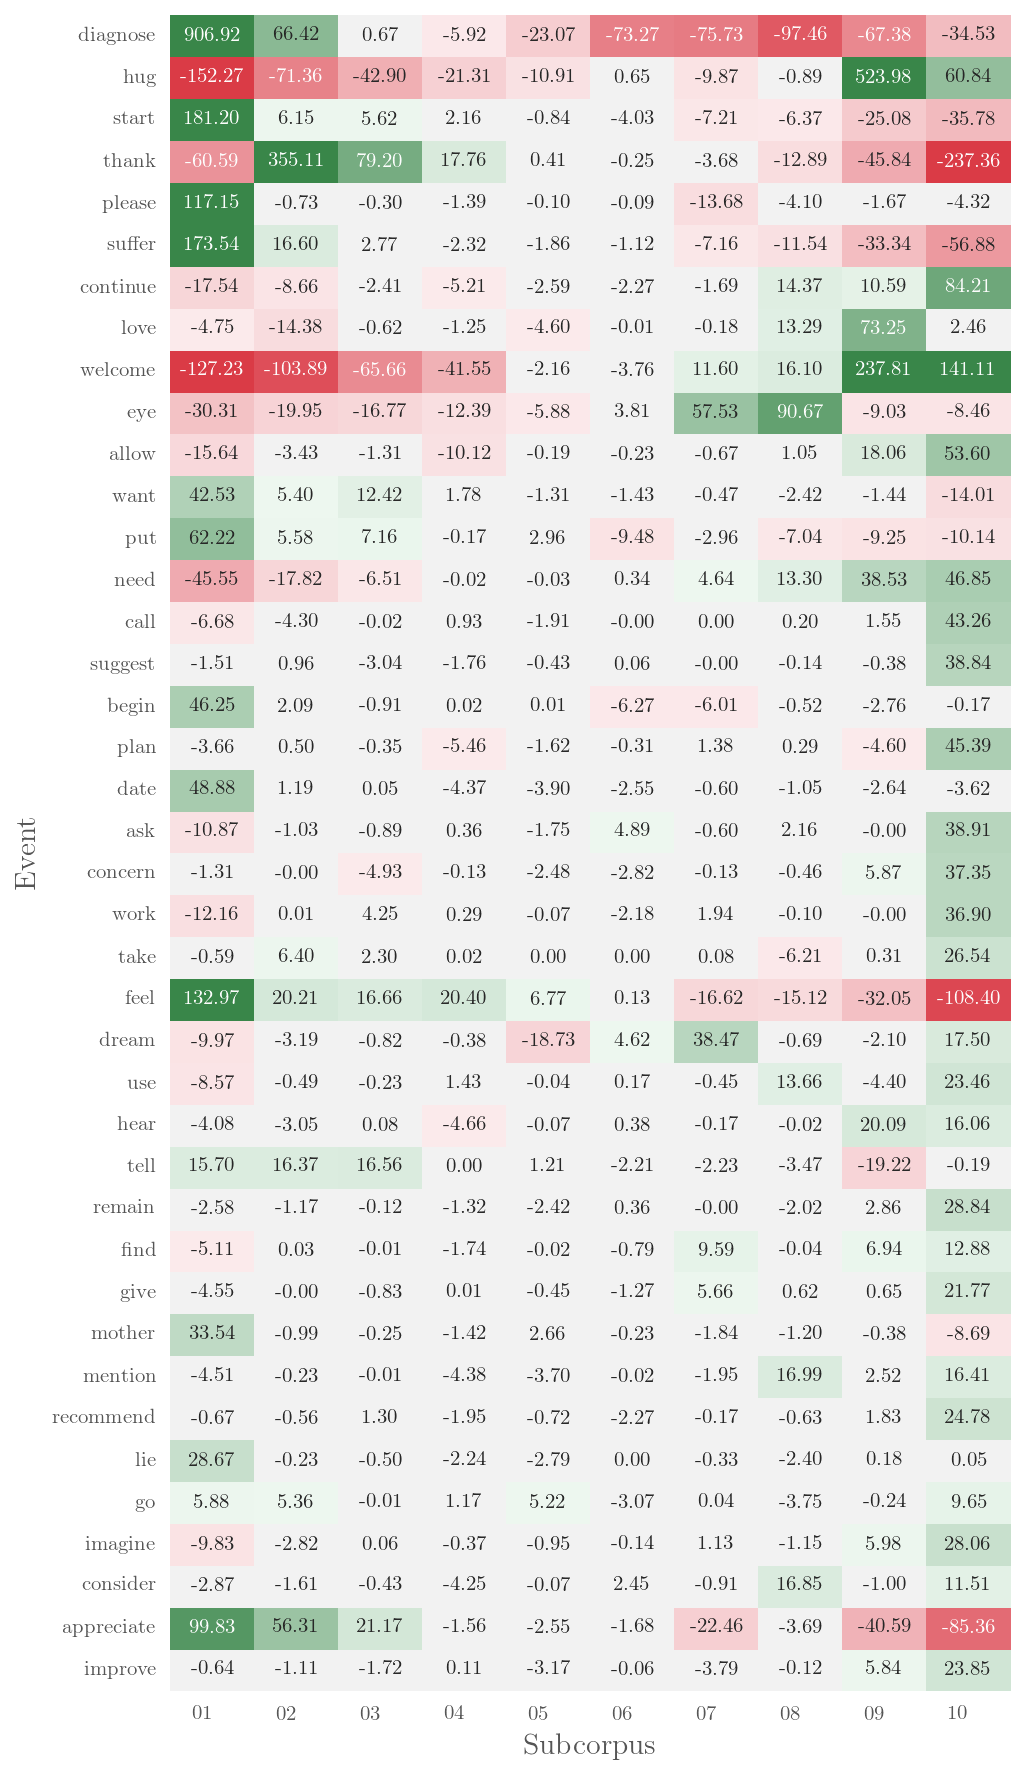
\includegraphics[width=0.80\textwidth]{images/event-heatmap.png}
    \hspace{1.6cm}
    \caption{Key and unkey Events in each subcorpus}
    \label{fig:event_heatmap}
 \end{figure}

Figure \ref{fig:event_heatmap} shows which Events are key in each subcorpus according to a log-likelihood comparison of the Forum contents as a whole. By far the most key process in any subcorpus is \emph{diagnose} in Subcorpus 01, as diagnosis is both the catalyst for visits to the site, and the main entry condition for participatory information and support exchange. Similarly, \emph{thank} is key in second post because users thank others for replies to their first. Other key Events in first post reveal different kinds of motivations for joining the community, including being \emph{told} that they may have bipolar, \emph{dates} with bipolar people, and \emph{beginning\slash starting} new medication regimens or manic\slash depressive cycles.

As with the analysis of participants, where veteran members orient toward more positive lexis, positive processes related to social support also become more common in veteran post (\emph{hug, thank, love, welcome}). Another focal point is processes urging others to carry on (\emph{continue, remain, improve}), which also have positive connotations. This contrasts with the negative sentiments inherent in \emph{suffer} (as in, \emph{to suffer from bipolar}), which is key in first post (see below for a more thorough treatment of the ways in which bipolar is ascribed to the self and others across membership stages). Finally, it is notable that \emph{thank} and \emph{appreciate} are unkey in the final stage of membership; the increased social status in the community means that platitudes, for veterans, are no longer obligatory to the same extent.

\subsection{Construing diagnosis} \label{sect:diag}

%Concordancing allows a window into the figures involving \emph{diagnose} in early and late stages of membership.

% Goal of \emph{diagnose} processes in three stages of membership
% Circumstances in \emph{diagnose} processes in three stages of membership
\begin{figure}[htb]
    \centering
    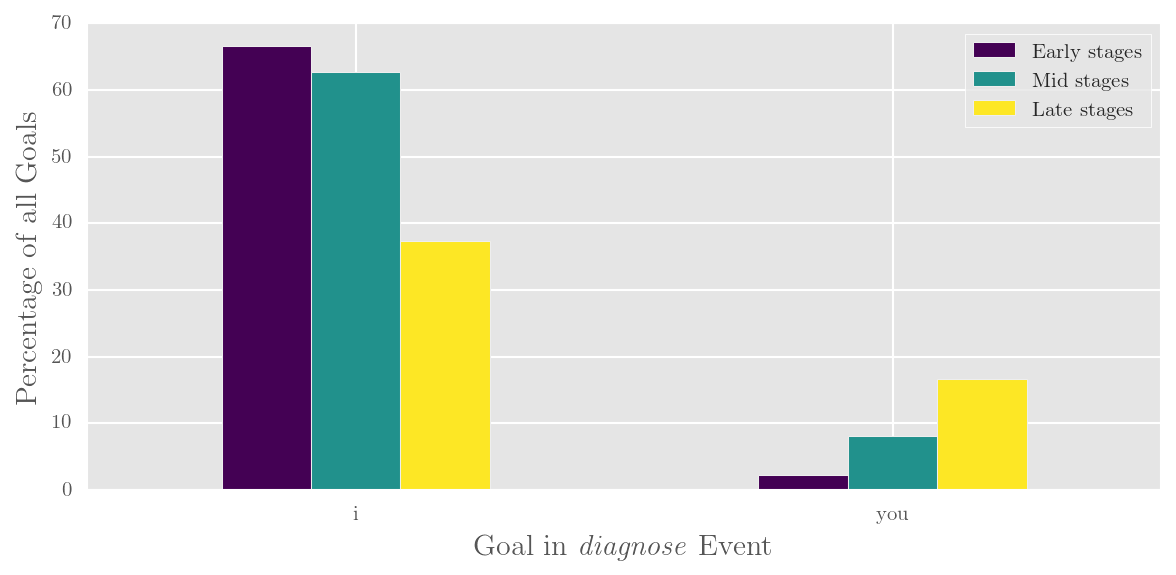
\includegraphics[width=0.8\textwidth]{images/goal-in-diag-ev.png}
    \caption[Goal of \emph{diagnose} processes]{Goal of \emph{diagnose} processes in three stages of membership}
    \label{fig:part_in_diag}
    \end{figure}

    \begin{figure}[htb]
    \centering
    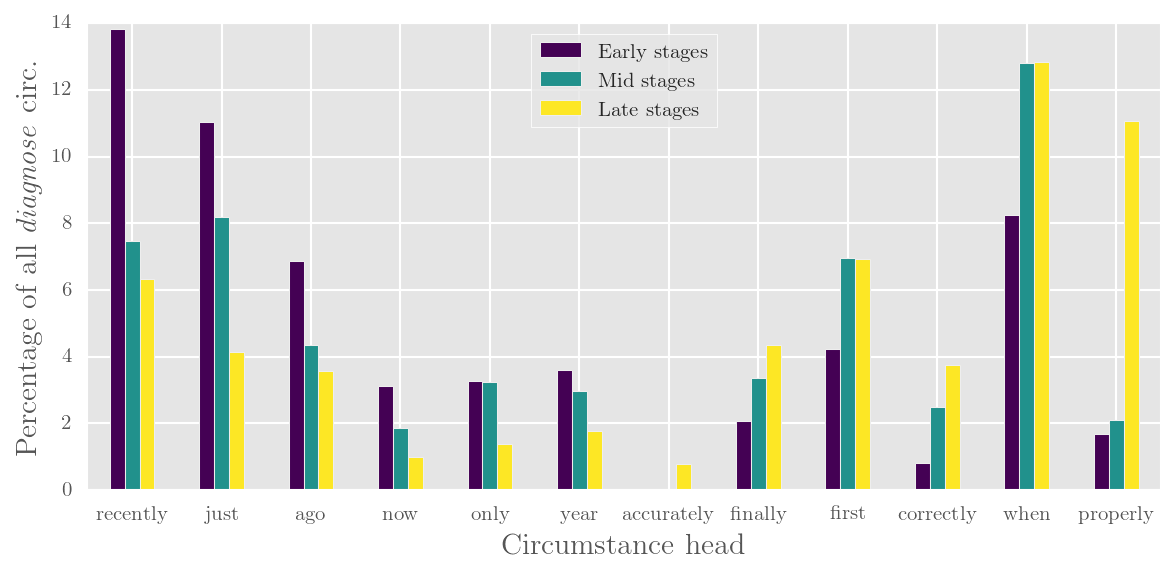
\includegraphics[width=0.8\textwidth]{images/diag-circ.png}
    \caption[Circumstances in \emph{diagnose} processes]{Circumstances in \emph{diagnose} processes in three stages of membership}
    \label{fig:circ_in_diag}
    \end{figure}

\emph{Diagnose} is a very prominent process in the Forum, and is by far the most key of key processes expressed in first post. By contrasting early, middle and late stages of membership, clear differences emerge in how the process of diagnosis is configured over time (Figure \ref{fig:part_in_diag}). Veteran members, for example, are more likely to represent the health professional as the Actor in the \emph{diagnose} process. In terms of circumstances (Figure \ref{fig:circ_in_diag}), there is a shift in focus away from temporal meanings, with veteran members instead framing the \emph{diagnose} process with regard to its correctness, accuracy and legitimacy. New members often enter the community because of a recent or possible future diagnosis. Veterans, on the other hand, seek to ensure that the diagnosis is reliable. This has the dual purpose of ensuring the legitimacy of the new member's `entry ticket', and ensuring conformance with the biomedical model, where successful treatment is predicated on accurate diagnosis. Indeed, a number of users enter the community not because of a diagnosis from a health professional, but because they are attempting to ascertain whether their self-diagnosis, or their informal diagnosis of a friend or loved one, can stand up to the scrutiny of lay-experts. Veteran members, however, are reluctant to legitimise these kinds of strategies, due to their deviation from a normative conceptualisation of the `correct' consumer journey.

%Furthermore, they frame diagnosis as possibilistic: diagnoses can be \emph{suspected} or \emph{unofficial}. Such a framing is at odds with the normative biomedical model, however: informal kinds of diagnosis cannot be acted upon with appropriate treatment regimens. Veteran members therefore stress correct diagnosis in order to realign new members' construal of diagnosis with the ideology of the board.

%Though the focus of the community is on offering information and support for people with bipolar}, those without official diagnoses ultimately cannot be helped \cite{vayreda_social_2009}. Ideologically, validation of community membership is withheld until new members have aligned with a normative biomedical trajectory that foremost involves diagnosis by professionals operating within a formal healthcare institution.

Notably, veteran members may deliberately undermine the biomedical model of diagnosis. While expressing conviction that diagnosis must be performed by a qualified health professional, they may simultaneously hint that the newcomer is \emph{probably} bipolar, or that non-bipolar diagnoses are in error. As was shown in the qualitative analysis in Chapter \ref{chap:introdata}, two separate replies to an undiagnosed newcomer relied upon the same lexicogrammatical means of hinting (\emph{It sounds like you might have bipolar to me}; \emph{if sounds very likely that you might have Bipolar disoder}), while nonetheless insisting on seeking diagnosis through mainstream channels (\emph{Find you a dr that can make a correct Diagnosis}; \emph{We aren't docs here and can't diagnose you}). As shown in the following section, in veteran--veteran interactions, health professionals' ability to correctly identify and treat people living with bipolar is occasionally into question. This keeps the membership entry point open for those who have initially failed to meet the core criterion of a legitimate diagnosis, while pushing undiagnosed, suspected bipolar users toward actions that are in line with mainstream medical norms. %Help can be better provided once the condition is met.

\subsubsection{Diagnosis and grammatical metaphor}

Grammatical metaphor entails the use of one grammatical component to do the work that is congruently performed by another. Nominalisation is one of the most common examples \cite{simon-vandenbergen_grammatical_2003}. What is congruently an action, process or Event (e.g. to \emph{applaud}) may be reconstrued as a participant (\emph{applause}), allowing denser packaging of information. Turning the process into a participant also facilitates taxonomisation and classification: the lexical component of a nominal group may include Classifier, Epithet and Numerative, in addition to the Thing; in the verbal group, the only lexical component is the Event \cite{halliday_introduction_2004}. This kind of grammatical metaphor also opens up the reconstrued process to deixis. For these reasons, it is a key characteristic of scientific English \cite{halliday1999construing}. 

Over the course of membership, the process of diagnosis undergoes a steady shift toward metaphorical realisation as a participant. In formal terms, it is more often nominalised. Figure \ref{fig:diag-gram-met} shows the strong relationship, but inexact, relationship between nominalisation and grammatical metaphor in the case of diagnosis: nominal and participant realisations become more frequent, while verbal and process realisations decrease. Charting experiential roles shows us that \emph{diagnose} is not limited to participant and process roles: commonly, it is a part of a circumstance (\emph{we received more help in terms of diagnosis and treatment}) or modifies a Thing (\emph{it is extremely common for those with undiagnosed bipolar disorder to self medicate}). The increasing extents to which \emph{diagnose} is nominalised, and to which \emph{diagnose} is represented as something other than a process, demonstrate an important discourse-semantic shift. By moving away from \emph{diagnose-as-process}, it becomes possible to represent diagnosis as a possession (\emph{it's great you have a final diagnosis and have started medication}), and therefore as something that can be acted upon or thought of in a particular way (\emph{i finally feel like i've accepted my diagnosis}). Another possibility opened up by nominalisation is the potential for modification through Epithets (\emph{this is a frightening diagnosis, particularly if you don't know anyone who has it}). Classification of \emph{diagnosis} through adjectival modification is also made possible (\emph{accurate}\slash \emph{correct} diagnosis), but, of course, as shown in Figure \ref{fig:circ_in_diag}, agnate meanings can be made through circumstantial modification of diagnose as a process (\emph{accurately\slash correctly diagnosed}). A final grammatical affordance is that diagnosis as a participant in a relational process can highlight its potential to be incorrect (\emph{my current diagnosis is schizo-affective disorder}; \emph{bp is becoming a catch-all diagnosis, frequently made by a well-meaning family doctor}). In this way, grammatical metaphor not only contributes to an increasingly scientised register, but also expands veteran members' ability to explain medical processes and their relationship to other members \cite{heyvaert_nominalization_2003}.

Calculating the relative frequencies of common modifiers of diagnose as verb (\emph{diagnose}, \emph{diagnosed}, \emph{diagnosing}) and diagnose as noun (i.e. diagnosis\slash diagnoses) clearly shows a preference for temporal modification of verbs and veracious modification of the nominal form (Table \ref{relfreq-diagnose-mods}).

%More generally, veterans may wish to invoke a scientised register, which 

% Grammatical metaphor in \emph{diagnosis}, via word classes and experiential roles
\begin{figure}[htb]
    \minipage{0.48\textwidth}\centering
    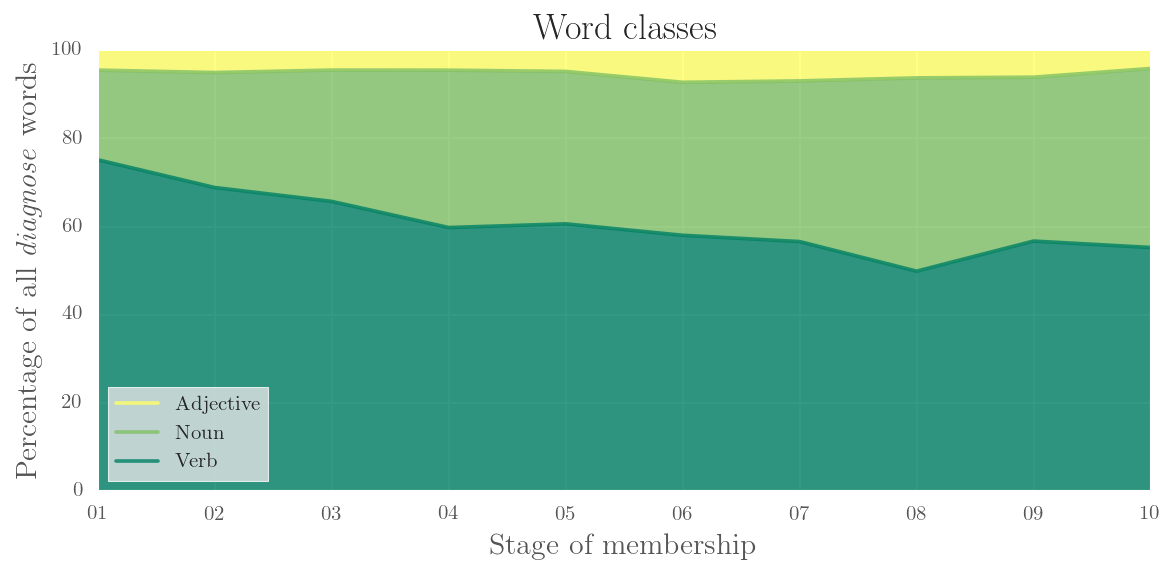
\includegraphics[width=1.00\textwidth]{images/wc-diag.png}
    \endminipage\hfill
    \minipage{0.48\textwidth}\centering
    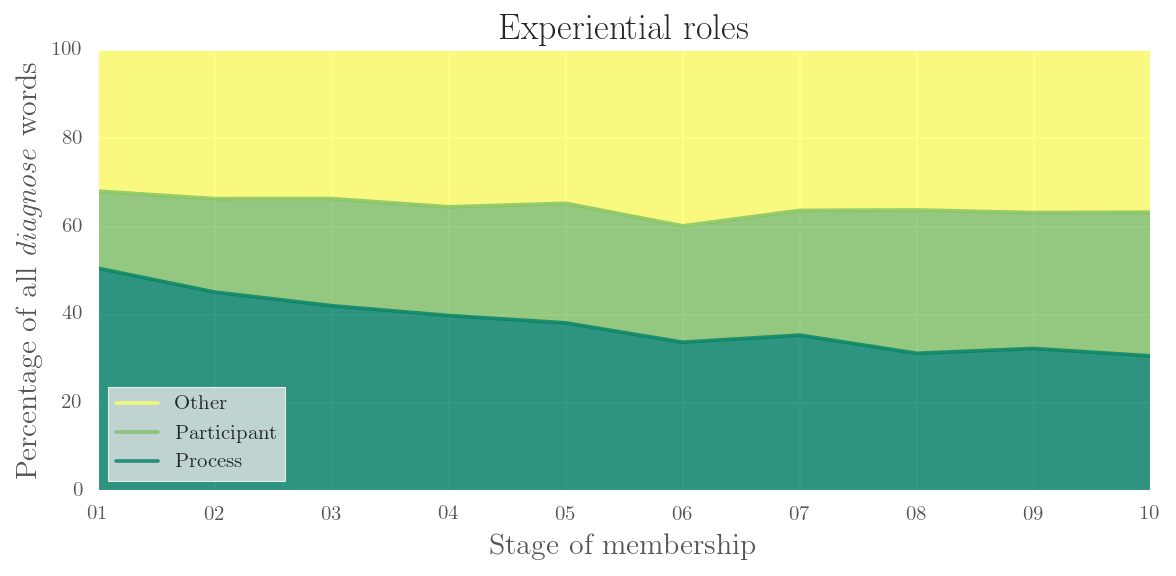
\includegraphics[width=1.00\textwidth]{images/exp-diag.png}
    \endminipage\hfill
    \caption[Grammatical metaphor in \emph{diagnosis}]{Grammatical metaphor in \emph{diagnosis}, via word classes and experiential roles}
    \label{fig:diag-gram-met}
    \end{figure}

\begin{table}[htb]
\begin{tabular}{lrlr}

\toprule
\emph{Diagnose}  & Rel freq.        & \emph{Diagnosis} & Rel. freq. \\
\midrule
not               &  11.80 & bipolar    &  11.13 \\
ago               &  11.10 & proper     &   8.82 \\
just              &   7.60 & correct    &   7.49 \\
recently          &   6.68 & dual       &   5.07 \\
when              &   4.16 & right      &   4.41 \\
now               &   3.54 & new        &   3.96 \\
only              &   3.11 & official   &   2.75 \\
properly          &   2.75 & different  &   2.64 \\
also              &   2.27 & wrong      &   2.20 \\
finally           &   2.12 & other      &   2.20 \\
so                &   2.09 & same       &   1.87 \\
never             &   2.09 & initial    &   1.65 \\
then              &   1.93 & possible   &   1.54 \\
correctly         &   1.50 & true       &   1.54 \\
well              &   1.47 & recent     &   1.43 \\
\bottomrule
\end{tabular}
\caption{Most common modifiers of \emph{diagnose} and \emph{diagnosis}}
\label{relfreq-diagnose-mods}
\end{table}

\section{Future directions}

This study has highlighted the utility of functional grammar and computational methods in interpreting online health discurse. At the same time, it demonstrates that many of the kinds of results that typically come from qualitative analysis can to some extent be automated, increasing reliability, reducing the potential for bias introduced either by researcher or sampling.

Because the methods for data collection and analysis are automated and open-source, reproducing the analysis pipeline on other communities is trivial. This would facilitate multilingual studies, or studies of different health conditions. Alternatively, using the methodoligcal pipeline developed here, focus could switch from \emph{diagnosis} to another key event in health journeys (such as \emph{relapse}, in a forum for substance abuse, or \emph{remission}, in a cancer community).

Finally, a number of more novel computational methods could potentially be used. While the focus of this study was on lexicogrammatical analysis of parsed data, methods such as topic modelling and word vectors could provide 

Given that these approaches typically do not involve annotation of text with theoretical models of language, they may well be an important step toward more complete automation of health language analysis.

\printbibliography[heading=bibintoc]

\end{document}